\documentclass[a4paper,pdflatex,11pt,mitminorthesis,singlespace,oneside]{cssethesis}
%% Language and font encodings
\usepackage[english]{babel}
\usepackage[utf8x]{inputenc}
%%\usepackage[section]{placeins}
\usepackage{booktabs}
\usepackage{tabu}
\usepackage[T1]{fontenc}
\usepackage{enumitem}
\usepackage{pgf,tikz}
\usepackage{mathrsfs}
\usetikzlibrary{calc}
\usetikzlibrary{arrows}
%% Sets page size and margins

%% Useful packages
%% Code 
\usepackage{listings}
\usepackage{url}
\usepackage{subcaption}
\usepackage{graphicx}
\usepackage{float}
\usepackage{cite}

%%Algorithm
\usepackage{amsmath}
\usepackage[linesnumbered,ruled]{algorithm2e}

% list source code
\usepackage{listings}
% list style definition
\lstdefinestyle{customc}{language=C++,
  basicstyle=\footnotesize\ttfamily,
  numbers=left,
  stepnumber=1,
  showstringspaces=false,
  tabsize=1,
  breaklines=true,
  breakatwhitespace=false,
  backgroundcolor=\color{black!5}, % set backgroundcolor
}
\lstset{escapechar=@,style=customc}

%%Theorem
\usepackage{amsthm}
\theoremstyle{remark}
\newtheorem*{remark}{Remark}
\newtheorem{theorem}{Theorem}[section]
\newtheorem{property}{Property}[section]
\theoremstyle{definition}
\newtheorem{definition}{Definition}[section]
\newtheorem{claim}[theorem]{Claim}
\newtheorem{proposition}[theorem]{Proposition}
\newtheorem{lemma}[theorem]{Lemma}
\newtheorem{corollary}[theorem]{Corollary}
\newtheorem{conjecture}[theorem]{Conjecture}

\thesisauthor{Shizhe Zhao}
\thesisauthorlastname{Zhao}
\thesisdepartment{Caulfield School of Information Technology}
%                  Clayton School of Information Technology is the default
\thesisauthorstudentid{27505928} % Needed for litreview
\thesisauthoremail{szha414\@@student.monash.edu} % Optional. Note that the @ is
											 % given as \@@. This is not
											 % necessary in normal LaTeX,
											 % but it is if you use the
											 % amsmath package - so why not
											 % get into the habit?
%\thesismonth{July} % Optional. Current month is used if this is not set
%\thesisyear{2002} % Optional. Current year is used if this is not set
\thesistitle{Fast Obstacle Spatial Query Processing on Navigation Mesh}
\thesissupervisor{Assoc. Prof. David Taniar}

\begin{document}

\frontmatter					% start the thesis front matter.
\thesistitlepage				% Generate the title page.
\thesiscopyrightpage			% Generate the copyright page.
%\thesisdedicationpage			% Generate a dedication page (optional)
\tableofcontents				% Generate a table of contents.
%\listoftables					% Generate a list of tables (optional).
%\listoffigures					% Generate a list of figures (optional).
\pagebreak

\begin{thesisabstract}			% generate the abstract page.
Obstacle k-Nearest Neighbours problem is the k-Nearest Neighbour problem in a 
two-dimensional Euclidean plane with obstacles (\emph{OkNN}).
Existing and state of the art algorithms for OkNN are based on incremental 
visibility graphs and as such suffer from a well known disadvantage: costly 
and online visibility checking with quadratic worst-case running times.
In this research we develop a new OkNN algorithm which avoids these disadvantages
by representing the traversable space as a collection of convex polygons; i.e.
a Navigation Mesh. 
We then adapt a recent and optimal navigation mesh algorithm, \textit{Polyanya}, from the
single-source single-target setting to the the multi-target case. 
We also give two new and online heuristics for OkNN.
In a range of empirical comparisons, we show that our approach can be orders of magnitude faster than competing methods that rely on visibility graphs.
The work has been accepted for publication in \textit{Proceedings of the 11th Annual Symposium on Combinatorial Search (SoCS’2018), colocated with
IJCAI/ECAI’2018, July 2018 (Shizhe Zhao, David Taniar, Daniel Harabor, "Fast OkNN on Navigation
Mesh")}.

\textit{Keywords}: Obstacle Nearest Neighbor, kNN, Navigation Mesh, Spatial Search, Obstacle
Distance, Obstacle Navigation

\end{thesisabstract}                 

%\thesisdeclarationpage			% generate the declaration page (optional).

\begin{thesisacknowledgments}	% generate the acknowledgements page (optional).
  Acknowledgement placeholder 
\end{thesisacknowledgments}  

%%%%%%%%%%%%%%%%%%%%%%%%%%%%%%%%%%%%%%%%%%%%%%%%%%%%%%%%%%%%%%%%%%%%%%%%%%%%%%
%%
%% Main matter 
%%
\mainmatter						% start the thesis body.

\chapter{Introduction}
\section{Overview}
Obstacle k-Nearest Neighbour (OkNN) is a common type
of spatial analysis query which can be described as follows:
given a set of target points and a collection of polygonal obstacles,
all in two dimensions, find the k closest targets to
an a priori unknown query point q. Such problems appear
in a myriad of practical contexts. For example, in an industrial
warehouse setting a machine operator may be interested
to know the k closest storage locations where a specific inventory
item can be found. OkNN also appears in AI planning domain, for example,
in competitive computer games, agent AIs often rely on nearest-neighbour information
to make strategic decisions such as during navigation,
combat or resource gathering.

\begin{figure}[htp]
  \centering
  \includegraphics[width=.7\linewidth]{./pic/obs_dis.png}
  \caption{\small
  We aim to find the nearest neighbour of point $q$ from among the set of target points $A,B,C,D$.
  Black lines indicate the Euclidean shortest paths from $q$.
  Notice $D$ is the nearest neighbor of $q$ under the Euclidean metric
  but also the furthest neighbor of $q$ when obstacles are considered.}
\label{obs_dis}
\end{figure}

Tradional kNN queries in the plane (i.e. no obstacles) is a well studied problem that can be
handled by algorithms based on spatial index. A key ingredient to the success of
these algorithms is the Euclidean metric which provides perfect distance information between
any pair of points. When obstacles are introduced however the Euclidean metric becomes an often
misleading lower-bound. Figure~\ref{obs_dis} shows such an example.

\section{Major Challenges}
Two popular algorithms for OkNN, which can deal with obstacles, are
\emph{local visibility graphs}~\cite{zhang2004spatial} and \emph{fast
filter}~\cite{xia2004fast}. Though different in details, both of these methods
are similar in that they depend on the incremental and online construction of 
a graph of co-visible points, and use \textit{Dijkstra} to compute shortest path.
Algorithms of this type are simple to understand, 
provide optimality guarantees and the promise of fast performance. 
Such advantages make incremental visibility graphs attractive to researchers 
and, despite more than a decade since their introduction, they continue to 
appear as ingredients in a variety of kNN studies from the literature; e.g. 
~\cite{gao2011efficient,gao2016reverse,gao2009continuous}.
However, incremental visibility graphs also suffer from a number of notable 
disadvantages including:

\begin{enumerate}
  \item online visibility checks;
  \item an incremental construction process that has up to quadratic space and time complexity for the worst case;
  \item duplicated effort, since the graph is discarded each time the query 
  point changes.
\end{enumerate}

In section~\ref{lrknn}, we will introduce these two algorithms with detail,
and discuss why they have such disadvantages.

\section{Major Objectives}
In this research, we develop a new method for computing \emph{OkNN} which avoids same
disadvantages in existing works. Our research extends an existing very fast point-to-point
pathfinding algorithm \emph{Polyanya} to multi-target case.

\section{Thesis Organisation}
The rest of the thesis is organised as follows:
\begin{itemize}
  \item In chapter~\ref{lreview}, we review related works in different area, includes: AI
    searching, spatial index and spatial query processing.
  \item In chapter~\ref{propsedalgo}, we introduce the proposed algorithms and discuss their
    behaviors, formal proof for correctness will be proveded.
  \item In chapter~\ref{empirical}, we provide experiment results to demonstrate the
    performance of propsed algorithms.
  \item In chapter~\ref{conclusionfuture}, we summarize our contributions and discuss future
    works.
\end{itemize}

\chapter{Literature Review}\label{lreview}
\section{Overview}\label{lroverview}
\section{AI Search}\label{lrai}
\section{Spatial Index}\label{lrindex}
\section{Obstacle k-Nearest Neighbor}\label{lrknn}
\section{Pathfinding on Navigation Mesh}\label{lrnav}
\section{Related Spatial Queries}\label{lrquery}

\chapter{Proposed Algorithms}\label{proposedalgo}
\section{Overview}\label{proposedoverview}
From the previous chapter, we have introduced a very fast point-to-point algorithm \textit{Polyanya}, 
in this chapter, we discuss how to effectively adapt \textit{Polyanya} for OkNN settings where
there are multiple candidate targets. In section~\ref{prob}, we introduce formal problem
statement and math notations; in section~\ref{mot}, we introduce two less efficient but very
straightforward solution to show the motivations of our proposed research;
section~\ref{intervalh} and \ref{targeth} present our research works which discuss the design of our algorithms and the correctness in theory.

\section{Problem Statement}\label{prob}
OkNN is a spatial query in two dimensions that can be formalised as follows:
\begin{definition}{Obstacle k-Nearest Neighbour (OkNN):}\newline
Given a set of points $T$, a set of obstacles $O$, a distinguished point $q$ and and an integer $k$: 
\textbf{return} a set $\text{kNN} = \{t | t \in T\}$ such that $d_o(q, t) \le d_o(q, t_k)$ for all $t \in \text{kNN}$.
\end{definition}

\noindent Where:
\begin{itemize}[leftmargin=+1cm]
\item $O$ is a set of non-traversable polygonal obstacles.
\item $T$ is a set of traversable points called \emph{targets}.
\item $q$ is a traversable point called the \emph{query point}.
\item $k$ is an input parameter that controls the number of nearest neighbours that will be returned.
\item $d_e$ and $d_o$ are functions that measure the shortest distance between two points, as discussed below.
\item $t_k$ is the $k^{th}$ nearest neighbour of $q$.
\item $h_p(n, t)$ is the \textit{h-value} in Polyanya for a given search node $n$ and a target
  $t$.
\end{itemize}
\noindent
Stated in simple words, the objective is to find the set of $k$ targets which are closest to $q$ from among all possible candidates in $T$.
When discussing distances between two points $q$ and $t$ we distinguish between two metrics:
$d_e(q, t)$ which is the well known Euclidean metric (i.e. ``straight-line distance'')
and $d_o(q, t)$ which measures the length of a shortest path $\pi_{q, t} = \langle q, \ldots, t\rangle$ between points $q$ and $t$ such that
no pairwise segment of the path intersects any point inside an obstacle (i.e. ``obstacle avoiding distance'').


\section{Motivation}\label{mot}
Since \textit{Polyanya} instantiates \textit{A*} search and since that algorithm is itself a
special case of \textit{Dijkstra}'s well know technique, there exists a simple modification at
hand: we can simply remove the influence of the cost-to-go heuristic and allow the search to
continue until it has expanded the $k^{th}$ target, let's call this \textbf{\textit{zero-heuristic}}.
All other aspects of the algorithm, including termination
\footnote{There are two cases to consider depending on whether the query and target points are in the same polygon or in different polygons.
Both are described in~\cite{cuicompromise}}, remain unchanged.

\begin{figure}[ht]
    \centering
    \includegraphics[width=.6\linewidth]{pic/suc.png}
    \caption{\small Example of successors from \cite{cuicompromise}.}
    \label{suc2}
\end{figure}

The version of \textit{Polyanya} we have just described is unlikely to be efficient. Without a
\textit{h-value} for guidance, nodes can only be prioritized by the \textit{g-value} of their
root point, which is settled at the time of expansion. However, the \textit{g-value} does not
reflect the distance between the root and its corresponding interval. For example, in
Figure~\ref{suc2}, all observable successors would have the same expansion priority. Thus we
may expand many nodes, all equally priomising but having distant intervals, and all before
reaching a nearby target node with a slightly higher \textit{g-value}.

Another naive adaption is repeatedly calling an unmodified point-to-point \textit{Polyanya}
search, from the query point and to each target, let's call this \textbf{\textit{brute-force
Polyanya}}, see in algorithm~\ref{brute}. It is obvious that this solution is
inefficient when targets are many, however, in chapter\ref{empirical} we will see it
outperforms other proposed algorithms in certain contexts. 
\begin{algorithm}[!htp]
  \input{./code/brute_polyanya.pseudo}
  \caption{Brute-force Polyanya}
  \label{brute}
\end{algorithm}
To deal with this problem we develop two online heuristics which can be fruitfully applied to OkNN:
\begin{itemize}
  \item The Interval Heuristic, which prioritizes nodes using the closest point from its
    associated interval.
  \item The Target Heuristic, which relies on a Euclidean nearest neighbour estimator to
    provide a target dynamically at the time of expansion.
\end{itemize}
Each of these heuristic is applied in the usual way compute a final expansion priority: 
$f(n) = \textit{g-value}(n) + \textit{h-value}(n)$. In the remainder of this chapter we explore
these ideas in turn.

\section{Interval Heuristic ($h_v$)}\label{intervalh}
In some OkNN settings targets are myriad and one simply requires a fast algorithm to explore
the local area. This approach is in contrast to more sophisticated methods which apply spatial
reasoning to prune the set of candidates. The idea we introduce for such settings is simple and
can be formalised as follows:

\begin{definition}
  Given search node $n=[I, r]$, the \textit{h-value} in Interval Heuristic $h_v(n)$ 
  is the minimal Euclidean distance from the root $r$ to the segment $I$.
\end{definition}

Applying the Interval Heuristic $h_v$ requires solving a simple geometric problem: finding the
closest point on a line. The operation has low constant time complexity and we apply
standard techniques. Algorithm~\ref{intervalsrc} shows an example.

\begin{algorithm}[!htb]
  \input{./code/interval.pseudo}
  \caption{Polyanya OkNN with interval heuristic}
  \label{intervalsrc}
\end{algorithm}

\begin{theorem}{\textbf{consistency of $h_v$}:}\label{nodescv}
  In interval heuristic, the $\textit{f-value}$ of successor node is not less than the $\textit{f-value}$ of the parent
  search node.
\end{theorem}

\begin{proof}
  In the interval heuristic, when the successor is a search node, its \textit{f-value}
  can be interpreted as a lower-bound of the length of path from
  $s$ to any point on the segment $I$ through root $r$, and since it is generated by pushing
  away from the parent search node, its \textit{f-value} is larger than \textit{f-value}
  of the parent search node. If successor is a target node, the \textit{f-value} is the the length
  of the corresponding path and not less than the parent search node (the two values are equal 
  when the target is on the segment $I$).%$\square$
\end{proof}

\begin{corollary}
  Expanding a target node corresponds to finding a shortest path.
\end{corollary}

\begin{proof}
  As per Theorem~\ref{nodescv}, when a final node is expanded there exists
  no remaining candidate on the open list which can reach the node with a smaller $f$-value.
\end{proof}

\section{Target Heuristic ($h_t$)}\label{targeth}
In some OkNN settings the set of target are few (i.e. sparse), or there is a filter on the
query, for example, the query is like "the nearest storage location where capacity $>=100$". 
In these cases, without a reasonable heuristic guide, it is possible to perform many redundant
expansions in areas where no nearest neighbor can exist, Figure~\ref{hv} shows an example. 
\begin{figure}[htp]
  \centering
  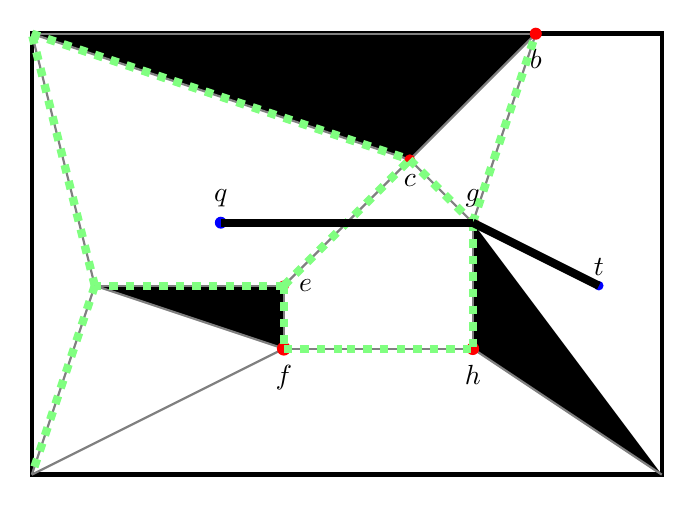
\begin{tikzpicture}[scale=0.8]
    %\coordinate (a) at (2, 6); 
\coordinate (a) at (0, 7);
\coordinate (b) at (8, 7); 
\coordinate (c) at (6, 5); 
\coordinate (d) at (1, 3);
\coordinate (e) at (4, 3);
\coordinate (f) at (4, 2);
\coordinate (g) at (7, 4);
\coordinate (h) at (7, 2);
%\coordinate (i) at (9, 0);
\coordinate (i) at (10, 0);
\coordinate (j) at (5, 2);
\coordinate (k) at (0, 7);
\coordinate (l) at (0, 0);
\coordinate (m) at (10, 0);
\coordinate (n) at (10, 7);
\coordinate (q) at (3, 4);
\coordinate (Q) at (3, 4);
\coordinate (t) at (9, 3);
\coordinate (o) at (7.5, 5.5);

\newcommand{\nodelabel}[2] {
    \node[fill,circle,scale=0.25,label=#2:$#1$,color=red] at (#1) {$#1$};
}

\newcommand{\medge}[2]{
    \draw[gray,thick] (#1)--(#2);
}

\newcommand{\vgedge}[2]{
    \draw[black,thick] (#1)--(#2);
}

\newcommand{\drawVs}{
    %\nodelabel{a}{above}
    \nodelabel{b}{below}
    \nodelabel{c}{below}
    
    %\nodelabel{d}{left}
    \nodelabel{e}{right}
    \nodelabel{f}{below}
    
    \nodelabel{g}{above}
    \nodelabel{h}{below}
    %\nodelabel{i}{below}
}

\newcommand{\drawmeshs}{
    \medge{a}{k},\medge{a}{d},\medge{a}{b},\medge{a}{c}
    \medge{b}{c},
    \medge{c}{g}
    \medge{d}{f},\medge{d}{l},\medge{d}{e}
    \medge{l}{f}
    \medge{e}{c},\medge{e}{f}
    \medge{f}{h}
    \medge{g}{h},\medge{g}{b}
    \medge{h}{i}
}

\newcommand{\drawobstacles}{
    \fill[black] (a)--(b)--(c)--cycle;
    \fill[black] (g)--(h)--(i)--cycle;
    \fill[black] (d)--(e)--(f)--cycle;
}

\newcommand{\drawstart} {
    % \fill[blue] (q) circle[radius=.5ex];
    % \node[above] at (q) {$q$};
    \node[fill,circle,scale=0.25,label=above:$q$,color=blue] at (q) {$q$};

}

\newcommand{\drawend}{
    \fill[blue] (t) circle[radius=.5ex];
    \node[above] at (t) {$t$};
}

\newcommand{\drawboundary}{
    \draw[black, ultra thick] (k)--(n)--(m)--(l)--cycle;
}

\newcommand{\showvisible} {
    \fill[lightgray] (c)--(e)--(d)--(a);
    \nodelabel{e}{right}
    \nodelabel{c}{below}
    \drawstart;
}

\newcommand{\stepa} {
    \fill[lightgray] (c)--(e)--(d)--(a);
    \fill[lightgray] (c)--(g)--(h)--(f)--(e);
    \draw[black, thin] (q)--(g);
    \draw[green, very thick] (e)--(c);
    \drawstart
    \drawVs
}

\newcommand{\stepb} {
    \fill[lightgray] (c)--(e)--(d)--(a);
    \fill[lightgray] (c)--(g)--(h)--(f)--(e);
    \fill[lightgray] (c)--(g)--(b);
    \draw[black, thin] (q)--(g);
    \draw[green, very thick] (e)--(c);
    \draw[black, thin] (g)--(t);
    \draw[black, thin] (q)--(g);
    \draw[green, very thick] (g)--(c);
    \draw[green, very thick] (g)--(b);
    \drawstart
    \drawend
    \drawVs
}

\newcommand{\polyanyaexpand}{
    \draw[black,very thin, dashed] (q)--($(q)!5cm!(e)$);
    \draw[black,very thin, dashed] (q)--($(q)!5cm!(c)$);
    \draw[orange!50, line width=3pt] (j)--(h);
    \draw[orange!50, line width=3pt] (h)--(g);
    \draw[orange!50, line width=3pt] (g)--(c);
    \draw[cyan, line width=3pt] (e)--(f);
    \draw[cyan, line width=3pt] (f)--(j);
}

\newcommand{\drawVG}{
    \vgedge{a}{d},\vgedge{a}{e},\vgedge{a}{g},\vgedge{a}{h}
    \vgedge{b}{g},\vgedge{b}{m}
    \vgedge{c}{d},\vgedge{c}{e},\vgedge{c}{g},\vgedge{c}{f},\vgedge{c}{h}
    \vgedge{d}{l},\vgedge{d}{g}
    \vgedge{e}{h},\vgedge{e}{n}
    \vgedge{f}{l},\vgedge{f}{h},\vgedge{f}{m}
    \vgedge{g}{n}
}
\newcommand{\drawmap}{
    \drawboundary
    \drawobstacles
    \drawmeshs
    \drawVs
    \drawstart
    \drawend
}

\newcommand{\intervalexpansion}{
    {\drawmap}
    {\draw[green!50, line width=3pt, dashed] (e)--(d);}
    {\draw[green!50, line width=3pt, dashed] (d)--(a);}
    {\draw[green!50, line width=3pt, dashed] (a)--(c);}
    {\draw[green!50, line width=3pt, dashed] (e)--(c);}
    {\draw[green!50, line width=3pt, dashed] (d)--(l);}
    {\draw[green!50, line width=3pt, dashed] (e)--(f);}
    {\draw[green!50, line width=3pt, dashed] (f)--(j);}
    {\draw[green!50, line width=3pt, dashed] (j)--(h);}
    {\draw[green!50, line width=3pt, dashed] (g)--(h);}
    {\draw[green!50, line width=3pt, dashed] (c)--(g);}
    {\draw[green!50, line width=3pt, dashed] (g)--(b);}
    {\draw[black, line width=3pt] (q)--(g);}
    {\draw[black, line width=3pt] (g)--(t);}
}
    \intervalexpansion
  \end{tikzpicture}
  \caption{\small Search space of Interval Heuristic:$q$ is query point,
  $t$ is a target, green dashed segments are the interval of expanded search nodes.
  From the figure we can see that the algorithm does unnecessary expansions in the direction that no target.}
  \label{hv}
\end{figure}
\noindent
In such cases more sophisticated spatial reasoning can help to prune the set of nearest
neighbours and guide the search. The idea we introduce for such settings can be formalised as
follows:
\begin{definition}\label{close}
  The closest target $t$ of a search node $n$ is $t \in T$ where $h_p(n, t)$ is minimum,
  the \textit{h-value} of search node $n$ in target heuristic is $h_t(n)=h_p(n,t)$.
\end{definition}

\begin{theorem}{\textbf{consistency of $h_t$}:}\label{nodesct}
In target heuristic, the $\textit{f-value}$ of successor node is not less than the $\textit{f-value}$ of the parent search node.
\end{theorem}

\begin{proof}
  Let the search node be $n=(I, r)$, the successor be $n'=(I', r')$, closest target of $n$
  be $t$, and the closest target of $n'$ be $t'$. 
  So we have $\textit{f-value}(n) = \textit{g-value}(r) + h_p(n, t)$, and 
  $\textit{f-value}(n') = g(r) + d_e(r, r') + h_p(n', t')$.
  According to definition of successor\cite{cuicompromise}, we have $r'=r$ or $r' \in I$.
  There are two cases:
  \begin{itemize}
    \item If $t=t'$, according to definition of $h_p$\cite{cuicompromise},
      we have $d_e(r, r') + h_p(n', t) >= h_p(n, t)$. 
    \item If $t,t'$ are different, according to definition~\ref{close},
      $h_p(n, t) <= h_p(n, t') <= d_e(r, r') + h_p(n', t')$.
  \end{itemize}
  Thus, $\textit{f-value}(n') >= \textit{f-value}(n)$.
\end{proof}

We implement this idea as follow: 
When the relative location between targets and $r$ are in case 3 of the $h_p$,
instead of flipping targets, we flip $r$, and thus formed six areas as shown in Figure~\ref{fa}.
For $t \in areaA$, the \textit{h-value} is $d_e(r, a) + d_e(a, t)$;
for $t \in areaA'$, the \textit{h-value} is $d_e(r',a) + d_e(a, t)$,
and because $d_e(r', a) = d_e(r, a)$, we can combine $areaA$ and $areaA'$,
so we need to find the nearest neighbor of $a$ for $t \in areaA \cup areaA'$;
by the same reason, we can combine $areaB, areaB'$, so finally we formed four areas.
Then following the example, we may reason as follows:
\begin{figure*}[!hbt]
  \centering
  \includegraphics[width=.7\linewidth]{pic/heuristic.png}
  \caption{
    \small  
    \textbf{(i)} In $areaA \cup areaA'$, $t_1$ is the nearest to $a$;
    \textbf{(ii)} in $areaB \cup areaB'$, $t_5$ is the nearest to $b$;
    \textbf{(iii)} in $areaC$, $t_3$ is the nearest to $r$;
    \textbf{(iv)} in $areaC'$, $t_7$ is the nearest to $r'$; 
  }
  \label{fa}
\end{figure*}
\begin{itemize}
  \item Suppose the next nearest target $t$ is in $areaA \cup areaA'$ (equiv. $areaB \cup areaB'$).
    Then the optimal path must pass through the point $a$ (equiv. $b$) so the minimum $h$-value can be computed as:
    $\mathbf{min}\{d_e(r, a) + d_e(t, a)\}$ such that $t$ in $areaA \cup areaA'$
    (equiv. $areaB \cup areaB'$).
  \item Alternatively, suppose the next nearest target $t$ is instead in $areaC$.
    Then the optimal path must pass through a point $p$ in the open interval $(a, b)$.
    So the minimum $h$-value can be computed by minimising across all target points in $areaC$.
    A similar argument applies to a next nearest neighbour in $areaC'$ and we can apply the same strategy,
    but only after mirroring the root point $r$ through the interval.
    This operation is in contrast to the heuristic used by Polyanya in the point-to-point setting,
    which mirrors the target through the interval.
\end{itemize}
\noindent
Identifying the candidate target with minimum $h$-value in each of the four cases can be improved,
from a linear-time operation to NN query, by storing all of the
targets in a spatial data structure such as $R^*$-Tree~\cite{beckmann1990r}.
Thus we may compute a lower-bound estimate to the next nearest neighbour by minimising over
four candidates returned by the $R^*$-tree instead of evaluating all possible target points.

\subsection{Further Refinements}
We may notice that the $h_t$ described thus far is potentially costly,
when compared to one constant time operation in $h_p$.
To mitigate this we could call $h_t$ less often. 
An observation is that a parent search node and its successor may use same closest target $t$
in their $h_t$. In this case, instead of running a new query, the successor can directly
inherit the $t$ from the parent.  We call this strategy \textit{lazy compute} and apply it throughout our experiments.
We find it reduces total number of node expansion by approximately 15\%.

\begin{corollary}\label{lazy-compute}
  Given search node $n=(I,r)$, its successor $n'=(I', r')$,
  and a target $t$ which is the closest target of $n$ among all possible candidates.
  Further suppose $\textit{f-value}(n)=\textit{f-value}(n')$ .
  Then $t$ is also the closest target of $n'$ among all possible candidates.
\end{corollary}

\begin{proof}
  If there is $t'$ closer to $n'$ than $t$, then $h_p(n', t') <
  h_p(n', t) = h_p(n, t)$, then 
  $$
  \textit{g-value}(r) + d_e(r, r') + h_p(n', t') < \textit{g-value}(r) + d_e(r, r') + h_p(n',
  t) = \textit{f-value}(n)
  $$
  so that $\textit{f-value}(n') < \textit{f-value}(n)$, which conflict with
  Theorem~\ref{nodescv}. Thus, such $t'$ doesn't exist.
  %$\square$
\end{proof}

Now, each search node has a target, and the search behavior should be broadly similar to 
the point-to-point setting.  But there is one significant difference:
when a nearest neighbor $t$ has been found, $t$ should no longer influence the search process.
Thus, we need to remove $t$ from search space and re-assign (i.e. update)
all search nodes in the queue which use $t$ as their closest target. 
To avoid exploring the entire queue we propose instead the following simple strategy: 
when such a node is dequeud from the open list, we apply $h_t$ to compute a new target
and we push the node back onto open all without generating any successors. 
We call this \textit{lazy reassign}.

\begin{lemma}\label{lazy-reassign}
  Let's call these search nodes who need reassignment \textbf{pseudo nodes}, and others
  \textbf{real nodes}. \textbf{Lazy reassign} never changes the relative order of real
  nodes in queue.
\end{lemma}

\begin{proof}
  Let $n_1, n_2$ be any pair of real nodes, and $s$ be any pseudo node.  After the reassignment,
  if $s$ become neither $n_1$ nor $n_2$, then inserting a third party search node has nothing to do with the relative order of $n_1$
  and $n_2$; otherwise, without the loss of generality, assume $s$ becomes $n_1$. If the relative
  order of them is $<n_2, s>$, then $\textit{f-value}(n_2) <= \textit{f-value}(s)$, and
  because of the definition~\ref{close}, we have $\textit{f-value}(s) <= \textit{f-value}(n_1)$, so
  relative order of $n_1, n_2$ doesn't change. Alternatively, if the relative order is $<s, n_2>$,
  then $n_1$  will be push to queue before $n_2$ pop out, so the relative order of $n_1, n_2$ doesn't
  change as well.%$\square$
\end{proof}

In Algorithm~\ref{hsearch}, we arrive at last at the final form of Polyanya OkNN. The algorithm
accepts either $h_v$ and $h_t$ as a heuristic function and has, in both cases, the same high level steps.

\begin{algorithm}[!ht]
  \input{./code/hsearch.pseudo}
  \caption{Polyanya OkNN}
  \label{hsearch}
\end{algorithm}

\section{Summary}
In this chapter, we start with two straightforward adaptions of point-to-point Polyany
and finally proposed two heuristics for the Polyanya OkNN algorithm.
For \textit{Interval Heuristic}, it supports multi-target by
removing $t$ from \textit{h-value}; for \textit{Target Heuristic}, it supports multi-target by
employing spatial index and computing closest target dynamically.
%Each heuristic has their
%suitable scenario, in following chapters, we will evaluate their performance under different
%scenarios (chapter~\ref{empirical})  and discuss some future improvements
%(chapter~\ref{conclusionfuture}). 

\chapter{Empirical Analysis}\label{empirical}
\section{Overview}\label{expoverview}
To evaluate Polyanya OkNN we consider two distinct setups and one large map with 
containing 9000 polygonal obstacles (this benchmark is described further in the next section).

In the first setup, targets are numerous and densely distributed throughout
the map. Our principal point of comparison in this case is \textit{LVG}~\cite{zhang2004spatial} which
is a state of the art method based on incremental visibility graphs. 
In the second setup, targets are few and sparsely distributed.
Our principal point of comparison in this case is \textit{brute-force Polyany}.
We motivate these decisions as follows:

\begin{itemize}[leftmargin=1cm]
\item When the map is large and targets are many (commonly the case in spatial database settings) \textit{LVG} considers only a small part of map and so its query processing can be very fast.
  \textit{Brute-force Polyany} meanwhile is infeasible to run (there are too many searches).

\item When the map is large targets are few ($<=10$) \textit{LVG} builds a visibility graph for almost entire map,
  and ends up with quadratic runtime complexity, which is unacceptable.
    Meanwhile, brute force \textit{Polyanya}, which is a very fast point-to-point pathfinding algorithm,
    can be competitive even when called repeatedly.
    This comparison is motivated by recent prior work involving kNN queries on road networks~\cite{abeywickrama2016k},
    where other fast point-to-point algorithms were shown to provide state-of-the-art performance in multi-targets scenarios,
    even when compared against dedicated kNN algorithms.
\end{itemize}
In both setups, we also include the Polyanya with \textit{zero-heuristic} as another baseline.
In all plots, the legend of competitors are:
\begin{itemize}
  \item \textit{Incremental Local Visibility Graph}\cite{zhang2004spatial}: \textit{LVG}
  \item \textit{Brute-force Polyanya}: \textit{BF Polyanya}
  \item \textit{Interval Heuristic}: \textit{OkNN-hv}
  \item \textit{Target Heuristic}: \textit{OkNN-ht}
  \item \textit{Zero-heuristic}: \textit{OkNN-h0}
\end{itemize}

In experiments, we examine performance based on elapsed time and expanded search node.
For \textit{LVG}, we count the number of expanded node in \textit{Dijkstra}.

The navigation mesh of map is generated by \textit{Constrained Delaunay Triangulation}, which is $O(nlogn)$;
the implementation of such algorithm is in library \textit{Fade2D} \footnote{http://www.geom.at/fade2d/html},
the total time on such preprocessing is about 6s.
We implemented in C++ the LVG algorithm (more details below) as well as two versions of multi-target Polyanya:
one each for Target and Interval Heuristic.
Our code is compiled with \textit{clang-902.0.39.1} using \textit{-O3} flag,
under \textit{x86\_64-apple-darwin17.5.0} platform.
All of our source code and test data set are  publicly available \footnote{http://bitbucket.org/dharabor/pathfinding}
All experiments are performed on a 2.5 GHz Intel Core i7 machine with 16GB of RAM and running OSX 10.13.4. 


\section{Implementation of \textit{LVG}}\label{imptlvg}
As discussed \textit{LVG} is our primary competitor in experiments with dense targets.
However, since there is no publicly available implementation, we write one ourselves.
We implement the method as per the description in the original paper~\cite{zhang2004spatial}.
The only differences is in construction of the visibility graph:
\textit{LVG} uses the rotational plane-sweeping algorithm from~\cite{sharir1986shortest} which runs worst case $O(n^2logn)$ time.
In our work we opted to simplify development complexity and use a $R^*$-tree\cite{beckmann1990r} query for visibility checking.
Each such query runs in $log(n)$ time  and we perform one check for each unique pair of vertices.
Thus the total complexity to build a visibility graph is also $O(n^2logn)$.
This implementation, as with the rest of our code, is made publicly available.

The implmentation of $R^*$-tree we use is also publicly available \footnote{https://github.com/safarisoul/ResearchProjects/tree/master/2016-ICDE-RkFN},
and appears in other recently published work~\cite{wang2016efficiently}.

\section{Benchmark}\label{dataset}

\begin{figure*}[!hbt]
  \centering
  \includegraphics[width=.7\linewidth]{pic/distribution.png}
  \caption{\small Example: a generated map with many targets. Color border polygons are
  obstacles, black crosses are targets.}\label{distribution}
\end{figure*}

The data set from our main competitor LVG\cite{zhang2004spatial}
is no longer available on the public Internet so we opt to generate new benchmark problems.
We extract the shape of all parks in Australia from \textit{OpenStreetMap}\cite{OpenStreetMap} and
use these shapes as polygonal obstacles. There are about 9000 such polygons in total.
Next we generate a map by tiling all obstacles in the empty square plane.
For the tiling, we first divide the square plane into grid having $\lceil\sqrt{|O|}\rceil$ number of rows and columns.
Then we assign each polygon to a single grid cell and normalize the shape of polygon by to fit inside the cell.
Figure~\ref{distribution} gives an example a map generated in this way.
For each experiment, we're using $1000$ random query points, grouping results by
\textit{x-axis}, and computing average; the size of each bucket is at least 10. 

One thing needs to be highlighted is that,
unlike \textit{LVG} ~\cite{zhang2004spatial} where obstacles are always rectangular,
we consider polygons of arbitrary shape, which is more realistic and potentially more challenging as there are more vertices to consider.
The total number of vertices across all polygons is more than 100,000. 

\section{Experiment 1: lower bounds on performance}\label{exp1}
\begin{figure*}[!htb]
  \begin{subfigure}{\linewidth}
    \begin{subfigure}{0.5\textwidth}
        \centering
        \includegraphics[width=.9\textwidth]{pic/e1_dense_time.png}
        \caption{}
        \label{e1_dense_time}
    \end{subfigure}%
    \hfill
    \begin{subfigure}{0.5\textwidth}
        \centering
        \includegraphics[width=.9\textwidth]{pic/e1_dense_gen.png}
        \caption{}
        \label{e1_dense_gen}
    \end{subfigure}
    \caption*{\small Dense experiment: $|T| \approx |O|,k=1$}
  \end{subfigure}\par\medskip
  \begin{subfigure}{\linewidth}
    \begin{subfigure}{0.5\textwidth}
        \centering
        \includegraphics[width=.9\textwidth]{pic/e1_sparse_time.png}
        \caption{}
        \label{e1_sparse_time}
    \end{subfigure}%
    \hfill
    \begin{subfigure}{0.5\textwidth}
        \centering
        \includegraphics[width=.9\textwidth]{pic/e1_sparse_gen.png}
        \caption{}
        \label{e1_sparse_gen}
    \end{subfigure}
    \caption*{\small Sparse experiment: $|T| = 5, k=1$}
  \end{subfigure}
  \caption{\small Experiment1: examine the performance when $dist$ increase, where
  $dist$ is the obstacle distance to retrieved target}
\end{figure*}

This experiment aims to examine the performance of proposed algorithms in the easiest case, which is $k=1$.
Results show that in dense targets scenario, the proposed algorithms outperform \textit{LVG} in both space and time (fig~\ref{e1_dense_time},\ref{e1_dense_gen}).

In the sparse targets scenario, \textit{target heuristic} has the smallest number of node
expansion (fig~\ref{e1_sparse_gen}), 
and both \textit{target} and \textit{interval} heuristic are outperformed on runtime by brute-force \textit{Polyanya} (fig~\ref{e1_sparse_time}) as $dist$ increases.
These results suggest the \textit{interval heuristic} has a large search space, and the
\textit{target heuristic} has a costly heuristic function. Results also show that \textit{brute-force Polyanya} is
not sensitive to $dist$, the reason is that it has to run a point-to-point search to all
targets no matter where the nearest neighbor is. 

\section{Experiment 2: computing more nearest neighbor}\label{exp2}
\begin{figure*}[!htb]
  \begin{subfigure}{\linewidth}
    \begin{subfigure}{0.5\textwidth}
        \centering
        \includegraphics[width=.9\textwidth]{pic/e2_dense_time.png}
        \caption{}
        \label{e2_dense_time}
    \end{subfigure}%
    \hfill
    \begin{subfigure}{0.5\textwidth}
        \centering
        \includegraphics[width=.9\textwidth]{pic/e2_dense_gen.png}
        \caption{}
        \label{e2_dense_gen}
    \end{subfigure}
    \caption*{\small Dense: $k \in [1,...10], |T| \approx |O|$}
  \end{subfigure}\par\medskip
  \begin{subfigure}{\linewidth}
    \begin{subfigure}{0.5\textwidth}
        \centering
        \includegraphics[width=.9\textwidth]{pic/e2_sparse_time.png}
        \caption{}
        \label{e2_sparse_time}
    \end{subfigure}%
    \hfill
    \begin{subfigure}{0.5\textwidth}
        \centering
        \includegraphics[width=.9\textwidth]{pic/e2_sparse_gen.png}
        \caption{}
        \label{e2_sparse_gen}
    \end{subfigure}
    \caption*{Sparse: $k \in [1,...10], |T|=10$}
  \end{subfigure}
  \caption{\small Experiment2: examine the performance when $k$ increase}
\end{figure*}
%
This experiment aims to examine the performance of algorithm when query becomes harder ($k$ increasing).
Results show that, in the dense targets scenario, the proposed algorithms still outpeform \textit{LVG}, even as $k$ increases (fig~\ref{e2_dense_time},\ref{e2_dense_gen}).
In the sparse targets scenario, results show that brute-force $Polyanya$ is not sensitive to $k$.
Meanwhile each of the two OkNN variants requires increasing amounts of node operations (and thus memory) and become quickly outperformed.
A side effect of \textit{target heuristic} when $k$ increase is that \textit{lazy reassign} causes extra node expansions.

\section{Experiment 3: changing number of targets}\label{exp3}

\begin{figure*}[!htb]
    \centering
    \begin{subfigure}{0.5\textwidth}
        \centering
        \includegraphics[width=.9\textwidth]{pic/e3_time.png}
        \caption{}
        \label{e3_time}
    \end{subfigure}%
    \hfill
    \begin{subfigure}{0.5\textwidth}
        \centering
        \includegraphics[width=.9\textwidth]{pic/e3_gen.png}
        \caption{}
        \label{e3_gen}
    \end{subfigure}
    \caption{\small Experiment 3: examine the performance when $|T|$ increase, $k=1, |T| \in [1,...10]$}
\end{figure*}

This experiment is run only on the sparse target set. It aims to examine the scalability of the proposed algorithms with an increasing
(but still sparse) number of targets.

Results show that proposed algorithms gradually outperform brute force \textit{Polyanya} in both time and node operations (fig~\ref{e3_time},\ref{e3_gen}).
This implies that the proposed OkNN variants algorithms are much better choices when the set of targets increase. 
Also notice that the node expansion decreases when $|T|$ goes large,
for \textit{interval heuristic}, the reason is that search nodes can reach target earlier; for
\textit{target heuristic}, in addition to previous reason, the \textit{R-tree} query in
heuristic function has good scalability. 
Although we have seen in other experiements that brute-force \textit{Polyanya} has an advantage when $k$ is large, this advantaged disappears as $|T|$ grows.
In some practical settings $|T|$ can be in the hundreds or thousands, e.g.~\cite{abeywickrama2016k} while $k$ is usually orders of magnitude smaller. 

\section{Analyze properties of target heuristic}\label{exp4}
From previous experiments, we notice that the \textit{target heuristic} always has smaller search space,
but it's sometimes orders of magnitudes slower than other competitors.
Thus, we want to dig out more properties of $h_t$.

Since $h_t$ is not design for the dense targets scenario,
we only consider experiment records from the sparse scenario,
and we analyze data in following aspects:
\begin{itemize}
  \item the ratio of the cost on the heuristic function in total elapsed time;
  \item the ratio of the reassignment in total expanded nodes;
  \item the ratio of the heuristic function call in total expanded nodes;
\end{itemize}.

\subsection{Ratio of heuristic cost}
Figure~\ref{hcost} shows the distribution of ratio:
$\textit{heuristic cost} / \textit{total cost}$.
\begin{figure*}[!htp]
  \centering
  \includegraphics[width=.5\linewidth]{./pic/hcost.png}
  \caption{}
  \label{hcost}
\end{figure*}
The result shows that the $h_t$ cost $\approx 90\%$ of total time, meaning that
\textit{target heuristic} needs at least an order of magnitude smaller search space 
to outperform competitors.

\subsection{Side effect}
A known side effect of $h_t$ is the \textit{reassignment} when $k>1$.
Figure~\ref{lazy_reassign} shows the ratio of $\textit{reassignment} / \textit{expanded nodes}$ when $k$ increase.
\begin{figure*}[!htp]
  \centering
  \includegraphics[width=.5\linewidth]{./pic/lazy_reassign.png}
  \caption{}
  \label{lazy_reassign}
\end{figure*}
The result shows that \textit{reassignment} happens more freqently when $k$
increase, meaning that \textit{target heuristic} is more suitable when $k$ is small.

\subsection{Ratio of heuristic call}
Figure~\ref{lazy_compute} shows the distribution of ratio:
$\textit{heuristic call} / \textit{expanded nodes}$.
\begin{figure*}[!htp]
  \centering
  \includegraphics[width=.5\linewidth]{./pic/lazy_compute.png}
  \caption{}
  \label{lazy_compute}
\end{figure*}
To ignore the side effect when $k>1$, this plot only considers those records with $k=1$.
The plot implies the effect of \textit{lazy compute} can reduce $\approx 15\%$ heuristic call in
the search.

\section{Summary}
This chapter is to evaluate proposed algorithms.
In the chapter, we've discussed the motivation of experiment design,
the benchmark problem, and results of the experiment.
From these experiements, we can see that proposed algorithms outpeform the state-of-the-art
orders of magnitudes, and between these proposed algorithms, they have different suitable
scenarios.

\chapter{Conclusion and Future Work}\label{conclusionfuture}
\section{Research Contributions}\label{contribution}

In this work, we consider efficient algorithms for OkNN:
the problem of finding $k$ nearest neighbours in a plane and in the presence of obstacles.
We describe three new OkNN algorithms, all based on Polyanya~\cite{cuicompromise},
a recent and very fast algorithm for computing Euclidean-optimal shortest paths in the plane.
The first variant involves brute force search (one query per target point).
The second and third variants involve running Polyanya as a multi-target algorithm but with added heuristic guidance.
We develop two new online and admissible heuristics for this purpose: the Interval Heuristic and the Target Heuristic.

We compare these variant algorithms against one another and against LVG~\cite{zhang2004spatial},
an influential and state of the art OkNN method based on incremental visibility graphs.
The headline result from our experiment is that Polyanya OkNN can be up to
\textbf{three orders of magnitude} faster than LVG.

Moreover, each of the three variants appears best suited to particular OkNN settings:
\textbf{brute-force Polyanya} is highly effective when the number of candidates is small (independent of $k$);
the \textbf{Interval Heuristic} works well when targets are many (again, independent of $k$);
the \textbf{Target Heuristic} works well when targets are few and $k$ is also small.

\section{Future Works}\label{future}
We also consider future works in following directions.
Firstly, due to the high performance of proposed algorithms, we believe they can be used to
speed up other types of spatial queries which need to compute obstacle distance,
as described in section~\ref{lrquery}.

Secondly, we can improve heuristic function in \textit{target heuristic}.
In experiments, we notice that the \textit{target heuristic} cost $\approx 90\%$ of
the total running time on NN query, and one possible way is combining four queries into one.
Besides, in the literature review, we mainly focus on \textit{R-tree} and its variants which
have good scalability on dimensions, however, in our case, the dimension is always two (maybe
three in 3D extension). Thus, other high-performance and low-dimension data structures may helpful,
e.g. \textit{KD-tree}\cite{ooi1987spatial} and
\textit{Locality-sensitive hashing}\cite{slaney2008locality}.

Thirdly, \textit{brute-force Polyanya} can be improved by smart pruning. We notice that
the \textit{brute-force Polyanya} sometime outperforms other proposed algorithms in sparse scenarios,
thus, instead of considering all targets,
a pruning strategy like \textit{fast filter}\cite{xia2004fast} may make it work in general
scenario.


\pagebreak
\bibliographystyle{plain}
\bibliography{refs}
\appendix
\chapter{Dataset}
\begin{figure}[htb]
  \centering
  \includegraphics[width=\linewidth]{./pic/poly9000.png}
  \caption{\small The map in experiments, it has nearly 9000 polygonal obstacles, and 10,000
  vertexes.}
\end{figure}
\chapter{Source Code}
\lstinputlisting[caption=extract shape of parks, label=park2poly]{./code/park2poly.h}
\newpage
\lstinputlisting[caption=generate targets, label=gentarget]{./code/genPoints.h}
\newpage
\lstinputlisting[caption=target heuristic, label=heuristic_function]{./code/heuristic}
\newpage
\lstinputlisting[caption=final OkNN, label=oknn]{./code/knnheuristic.cpp}
\newpage

\end{document}
